% vim:ft=tex:
%
\documentclass{beamer}
\usepackage{graphicx}

\title{
	Denial of Service Attacks
}
\author{
	Andrew DeMaria (muff1nman) --- \texttt{ademaria@mines.edu}
}

\begin{document}
\maketitle
\begin{frame}{Introduction}
	\begin{columns}
		\begin{column}{0.3\textwidth}
			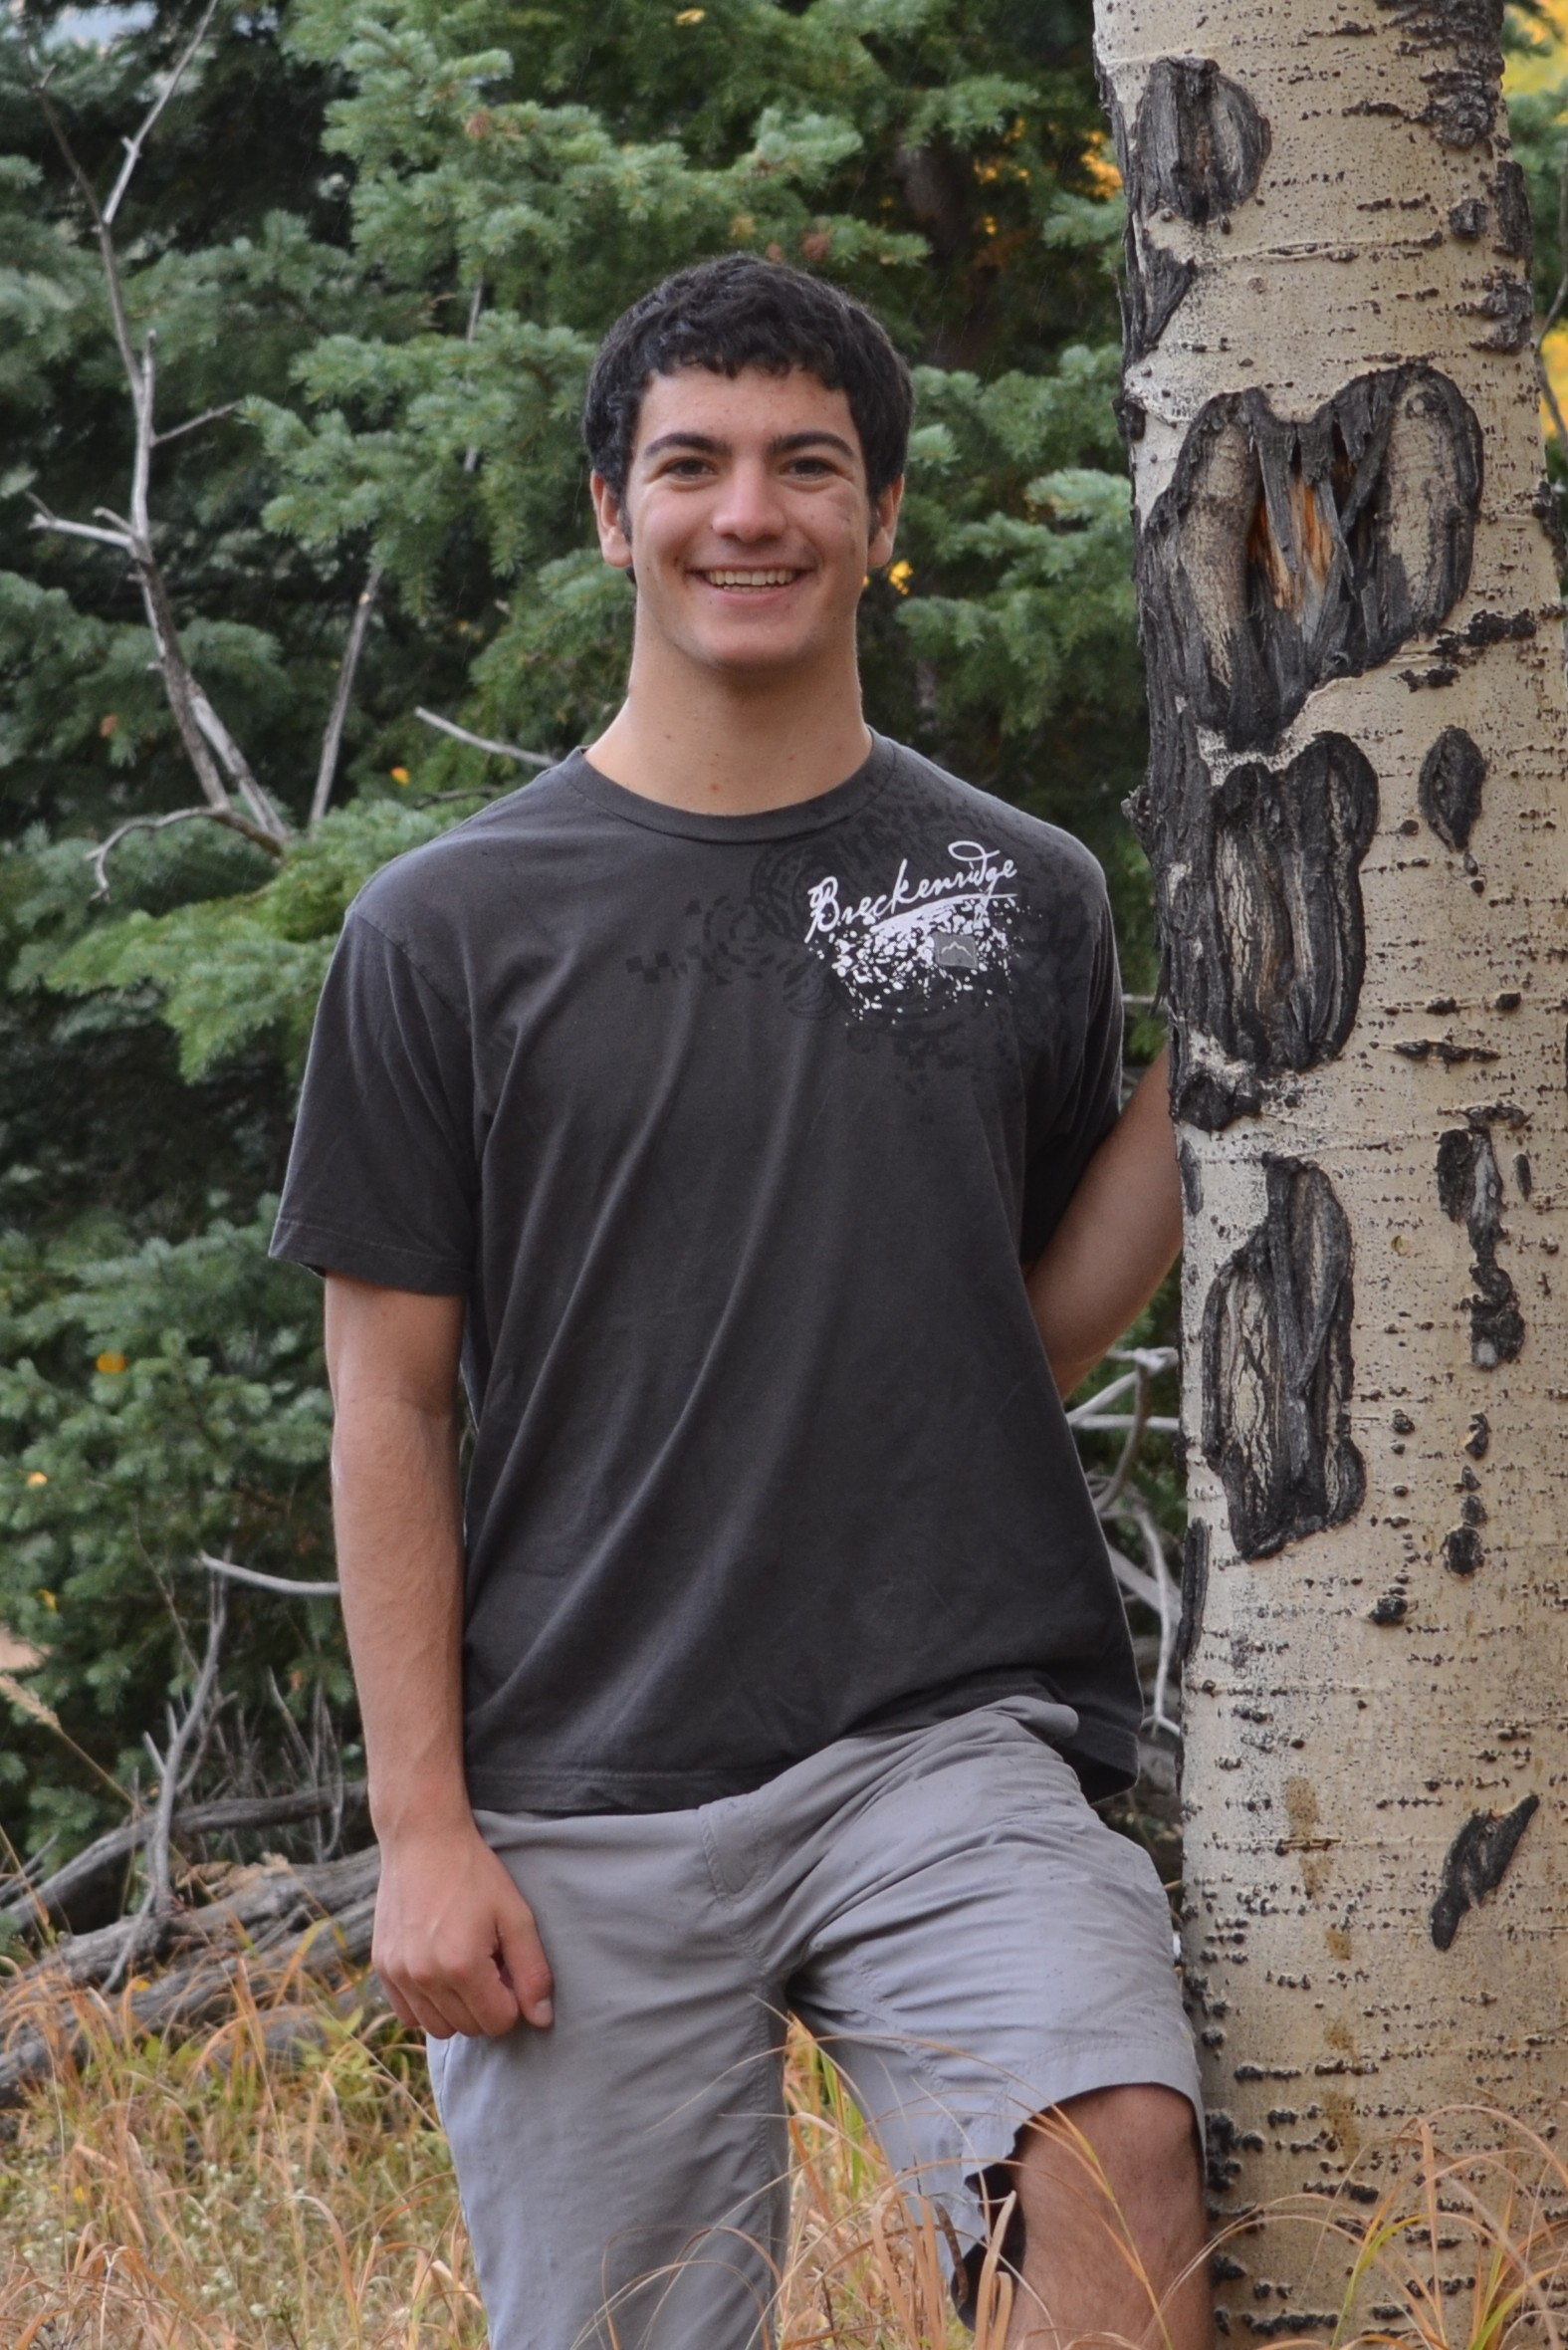
\includegraphics[width=1\textwidth]{images/andrew.JPG}
		\end{column}
		\begin{column}{0.7\textwidth}
			Andrew DeMaria is a senior at Colorado School of Mines in Golden, Colorado
			studying Computer Science. He spent 3 years teaching Cub Scouts at Peaceful
			Valley Ranch as a lifeguard. Afterwards, he was an intern for Lockheed Martin
			under their classified Military Support Program (MSP) where he worked on
			implementing a full Kerberos and LDAP based Authentication and Authorization
			system. There began his interest in information security and he has continued
			diving into the topic since.

			In his spare time, Andrew enjoys the Colorado Wilderness with backpacking,
			climbing, mountaineering, skiing and photography. When the weather does not
			cooperate he likes to hack on a Raspberry Pi.
		\end{column}
	\end{columns}
\end{frame}

\begin{frame}{Agenda}
	\begin{itemize}
		\item Background
			\begin{itemize}
				\item OSI model
				\item TCP/IP
				\item DNS
			\end{itemize}
		\item General Overview
			\begin{itemize}
				\item Purpose
				\item The people behind these attacks
				\item Events in the news
				\item Short History ?
			\end{itemize}
		\item Layer 2 Attacks
			\begin{itemize}
				\item :(
			\end{itemize}
		\item Layer 3 Attacks
			\begin{itemize}
				\item{SYN Food}
				\item{DNS Reflection}
			\end{itemize}
		\item Application Layer Attacks
			\begin{itemize}
				\item :(
			\end{itemize}
		\item Prevention
	\end{itemize}
\end{frame}


\end{document}

